Most static analyses can help find \emph{bugs} but cannot prove their absence (Astr\'ee is perhaps the outlier here).
%
These analyses can certainly be useful, but they do not cover a topic of ever-increasing importance: security.
%
Run-time monitors exist for enforcing security policies~\citep{ianjohnson:Erlingsson:2004:IRM:997617}, but fail late and impose significant overhead.
%
A \emph{sound} analysis that predicts that such run-time monitors never lead to an error state has given us two things:
\begin{itemize}
\item{\emph{proof} that our program is secure with respect to the monitored properties, and}
\item{a guarantee that we can safely remove the run-time monitor to improve performance.}
\end{itemize}
A \emph{precise} analysis is able to rule out enough spurious behavior that such predictions are actually possible in practice.
%
An analysis that says,
\begin{center}
  \textit{Nothing is true, everything is permitted}
\end{center}
is sound, but is so imprecise that we have learned nothing about the program's behavior. 
%
If security is not your goal, we still advocate a best-effort-soundness design strategy\footnote{So-called ``soundiness'' (\url{http://soundiness.org})}.

The question of sound versus unsound is a question of predicted behavior: are all states a program might find itself in considered?
%
A programming language semantics is the set of rules that determine how a program state evolves.
%
If we represent each program state as a node in a graph, and track evolution steps as edges, we get closer to the age-old \emph{control-flow graph} (AKA \emph{flow-chart}), but these concepts are shadows, projections, \emph{approximations} of concrete program behavior.
%
The art and science of static analysis design is the way we represent this graph of states; how little or how much detail we choose to represent in each state determines the precision and, often, the \emph{cost} of such an analysis.
%
The AAM methodology for static analysis design is a systematic augmentation of a given programming language semantics; this makes much of static analysis construction mindless boilerplate so that you can focus on your art -- hone in on the novelty of your abstraction.
%
First-order data-structures, numbers, arrays all have an abundance of literature for precise and effective approximations, so this paper focuses on higher-order data: closures and continuations, and their interaction with state evolution.
%

\paragraph{Example exemplifying why pushdown (return flow) matters}
Higher-order programs often create proxies, or monitors, to ensure an object or function interacts with another object or function in a sanitized way.
%
One example of this is with behavioral contracts on higher-order functions~\citep{dvanhorn:Findler2002Contracts}.
%
Simplified, here is how one might write an ad-hoc \texttt{int -> X} contract monitor, for some checkable property \texttt{X}:
\begin{center}
 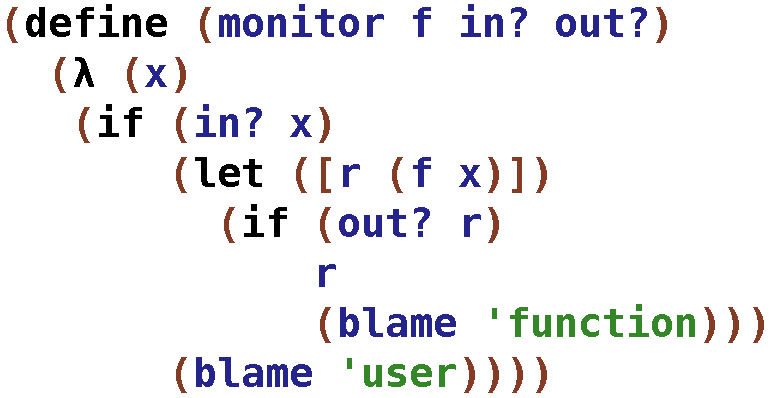
\includegraphics[scale=0.45]{monitor}
\end{center}
It is well known that $\eta$-expansion (wrapping functions) like this thwarts the precision of regular \zcfa{} and higher \kcfa{} as more wrappings are introduced.
%
In the case of this innocent program that operates on some list \texttt{$\ell$},
\begin{center}
 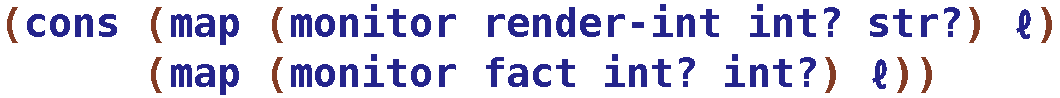
\includegraphics[scale=0.45]{pair}
\end{center}
the call to the wrapped factorial function within the second \texttt{map} reportedly returns to within the first \texttt{map}, according to \zcfa{}.
%
Add more contract wrappers and each $k$ for \kcfa{} is equally defeatable.
%
A pushdown abstraction that properly matches calls and returns has no trouble.
%
The control cycle from the second \texttt{map} to the first fools state-of-the-art termination checking for untyped higher-order languages~\citep{ianjohnson:DBLP:conf/aplas/SereniJ05}, as it depends on the product of \zcfa{}!
%
Termination-checking is necessary for interpreting portions of code as their logical equivalents.
%
Logical interpretations of code let us utilize high-performance theorem provers to test feasability of some code paths for greater precision~\citep{liquid-haskell}.
%
Functions can become deeply wrapped when interacting through several contracted modules, so pushdown models are nearly a requirement for hope at proving termination.